
\section*{IP und Netzwerkkonzepte}


\subsection*{Router}

Verbinden Netzwerke und Übertragungstechnologien miteinander, Paketweiterleitung
bis zum Ziel


\subsubsection*{Vorteile und Nachteile von Routern über Bridges:}

\begin{tabular}{|l||l|l|}
\hline 
\begin{tabular}{|c|}
\hline 
VORTEILE\tabularnewline
\hline 
\hline 
optimaler Pfad\tabularnewline
\hline 
Netze können logisch getrennt werden\tabularnewline
\hline 
Abgrenzung von Schicht 2 (Broadcast-Shit-Storm)\tabularnewline
\hline 
\end{tabular} & %
\begin{tabular}{|c|}
\hline 
NACHTEILE\tabularnewline
\hline 
\hline 
Teuer\tabularnewline
\hline 
konfigurationsintensiv\tabularnewline
\hline 
teilweise lassen sich Protokolle nicht routen (Netbios)\tabularnewline
\hline 
\end{tabular} & \multirow{1}{*}{%
\begin{tabular}{|c|c|c|}
\hline 
Kriterium & Router  & Bridge \tabularnewline
\hline 
\hline 
Loop-Unterdrückung & soso & Ja\tabularnewline
\hline 
Sicherheit & soso & soso\tabularnewline
\hline 
Pfade & optimiert & normal\tabularnewline
\hline 
Broadcast & intransparent & transparent\tabularnewline
\hline 
Multi MTU & Ja & Nein\tabularnewline
\hline 
Multi Medium & Ja & Nein\tabularnewline
\hline 
S3-unabhängig & Nein & Ja\tabularnewline
\hline 
 &  & \tabularnewline
\hline 
 &  & \tabularnewline
\hline 
\end{tabular}}\tabularnewline
\hline 
\end{tabular}


\subsubsection*{Routingalgorithmen:}
\begin{itemize}
\item RIP: Routing Information Protocol
\item BGP: Border Gateway Protocol
\end{itemize}

\subsubsection*{Brouter}
\begin{itemize}
\item Router mit Bridging-Funktionen, Bridges die routen
\end{itemize}

\subsubsection*{Gateway}
\begin{itemize}
\item Spannen über alle OSI Layer
\item Verbinden komplette Systeme
\end{itemize}

\section*{Internet Protocol}

Das IP Protokoll ist aus dem ARPANET (US DOD) entstanden. Idee: keine
zentrale Steuerung Der Internetlayer ist ein verbindungsloser Networklayer,
er ermöglicht Datengramme über jedes Netz zu senden. Der Transport-Layer
befindet sich oberhalb des Internet-Layers. Er beinhaltet die Kommunikation
zwischen der Quelle und dem Ziel.
\begin{itemize}
\item TCP Transmission Control Protocol

\begin{itemize}
\item Verbindungsorientiert, zuverlässig, Flowcontrol, fehlerfreie Übertragung
\end{itemize}
\item UDP User Datagram Protocol

\begin{itemize}
\item TCP ohne Flowcontrol, unzuverlässig, time-reliable
\end{itemize}
\end{itemize}
Der höhere Layer (Application Layer) beinhaltet Protokolle wie SSH,
HTTP etc.


\subsubsection*{Adressierung}

\begin{tabular}{|c|c|c|c|}
\hline 
Adresse & Dezimal & Binär & Berechnung\tabularnewline
\hline 
\hline 
Host-Adresse & 160.85.17.161 & 1010 0000 / 0101 0101 / 0001 0001 / 1010 0001 & \tabularnewline
\hline 
Netz-Adresse & 160.85.17.160 & 1010 0000 / 0101 0101 / 0001 0001 / 1010 0000 & host AND netmask\tabularnewline
\hline 
Netzmaske & 255.255.255.240 & 1111 1111 / 1111 1111 / 1111 1111 / 1111 0000 & \tabularnewline
\hline 
Broadcast-Adresse & 160.85.17.175 & 1010 0000 / 0101 0101 / 0001 0001 / 1010 1111 & host OR inv(netmask)\tabularnewline
\hline 
\end{tabular}%
\begin{tabular}{|c|c|}
\hline 
SubNetBin & SubNetDec\tabularnewline
\hline 
\hline 
0000.0000 & 0\tabularnewline
\hline 
1000.0000 & 128\tabularnewline
\hline 
1100.0000 & 192\tabularnewline
\hline 
1110.0000 & 224\tabularnewline
\hline 
1111.0000 & 240\tabularnewline
\hline 
1111.1000 & 248\tabularnewline
\hline 
1111.1100 & 252\tabularnewline
\hline 
1111.1110 & 254\tabularnewline
\hline 
1111.1111 & 255\tabularnewline
\hline 
\end{tabular}

Eine IP Adresse besteht somit aus 4Byte. Ebenfalls ist die IP 127.0.0.1
(/8) eine LoopBack Adresse (Bereich)


\subsubsection*{Classful-Routing}

Es wird keine SUbnetzmaske benötigt. A(2\textasciicircum{}24, 1byte
Netz (128), 3byte host (16’777’214)), B(2\textasciicircum{}16, 16’384,
65’534),C(2\textasciicircum{}8, 2’097’152, 254), D(Multicast,224.0.0.0
– 239.255.255.255), E(Zukunft, 240.0.0.0 – 247.255.255.255)


\subsubsection*{Routing}

Routen können mit ``route -n'' oder ``netstat -rn'' angezeigt
werden. (route add -net 160.85.19.0 netmask 255.255.255.0 dev eth2)
Falls kein Eintrag der Routingtabelle matcht, dann wird das Paket
einfach an den ``default'' Host weitergeleitet.


\subsection*{IP Protokoll}

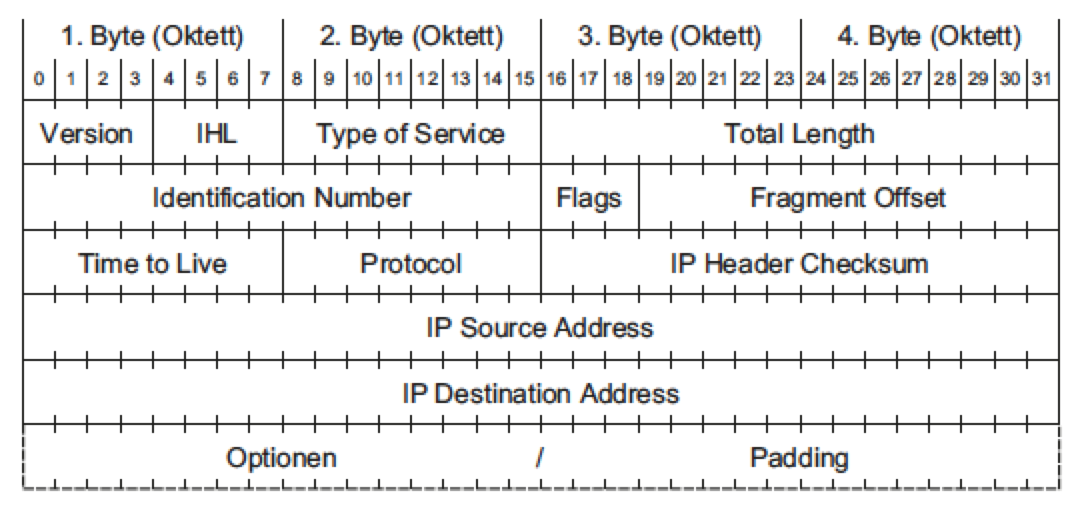
\includegraphics[width=7cm]{part2/ipheader}
\begin{itemize}
\item Die Internet Header Length (IHL) gibt die Länge des IP-Headers(min5/max15)
inklusive dem optionalen Teil(max40byte) in Double Words (32 Bit)
an. Die Länge bezeichnet also die Stelle wo im Datagramm die Nutzdaten
beginnen.
\item Quality of Service, gibt die Eigenschaft an. Dringend, hi reliablility,
throughput etc.
\item Total Length bezeichnet die gesamte L¨ange des Datagramms in Byte
(inklusive Header und Nutzdaten)
\item alle Fragmente des Datagramms den gleichen Identifikationswert
\item Flags: reserved null, fragment allowed, last more fragments
\item innerhalb des Datagramms ein Fragment: Der Fragment-Offset wird in
8-Byte-Einheiten (64 bits) angegeben, wobei das erste Fragment einen
Offset von Null hat (in maximal 213 = 8192 Fragmente zerlegt)
\item TTL: verbleibende Zeit in Sekunden an, die das Datagramm noch im Internet-System
verbleiben darf
\item Protocol: 1 ICMP / 6 TCP / 17 UDP
\end{itemize}

\subsubsection*{Fragmenting}

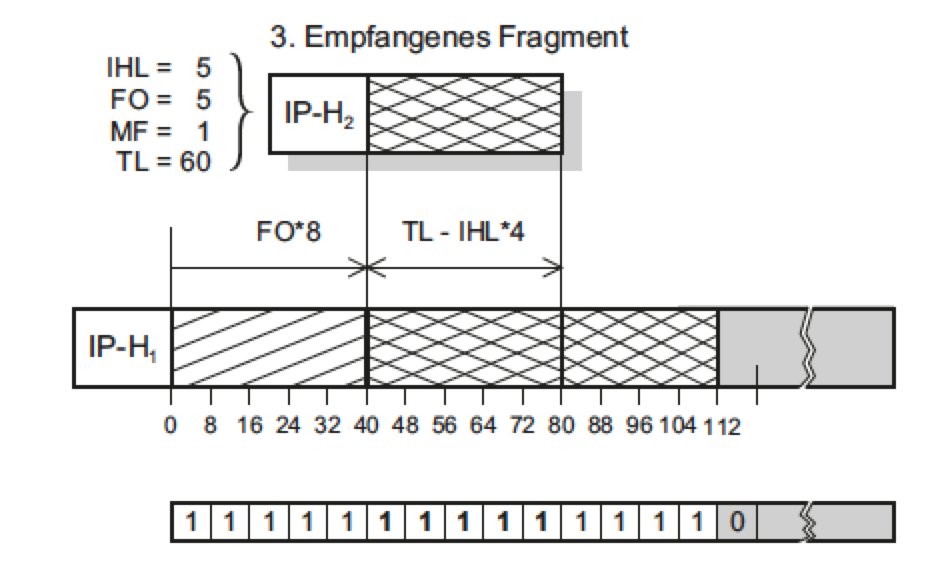
\includegraphics[width=6cm]{part2/fragmenting}


\subsubsection*{Adressauflösung}


\paragraph*{Address Resolution Protokoll (ARP)}

von 4-Byte-langen IP-Adressen auf 6-Byte-lange Ethernet-Adressen
\begin{itemize}
\item ARP-Request: ``who-has x.x.x.x'' als Broadcast ins Netz, wird durch
Bridges nicht gefiltert, dadurch kann hoher Traffic entstehen
\item ARP-Response''is-at y:y:y:y:y:y direkt an den anfragenden Knoten,
man beachte, dass die gesuchte Antwort im Feld Sender-MAC-Address
zu finden ist
\end{itemize}
Im ARP-Cache werden die Adressen zwischengespeichert, sodass man nicht
immer für jedes Paket eine neue ARP Anfrage machen muss. 
\begin{itemize}
\item Gratuitous ARP: ARP Requests/Replies die nich (nach Standart) notwendig
sind. Sie werden verwendet um IP-Adresskonflikte zu erkennen. Auch
beim ändern der IP-Adresse verschickt, aber mit dem Zweck, die ARP-Cache
der anderen Knoten zu berichtigen.
\end{itemize}
Mit dem Befehl ``arping -C 1 -U x.x.x.x'' kann ein Request gesendet
werden. 


\paragraph*{Reverse Address Resolution Protocol (RARP)}

von Ethernet-Adresse auf IP-Adresse
\begin{itemize}
\item Verwendung von RARP ist besser als das Ablegen einer IP-Adresse in
einem Disk-Image, weil dadurch die gleiche Konfiguration auf allen
Maschinen benutzt werden kann
\item Nachteil, dass es MAC-Layer-Broadcast benutzt, um den RARP-Server
-> von Routern nicht weitergegeben 
\item Alternative: BOOTP und DHCP\end{itemize}

